%
% Draft  document crimptype2.tex
% Classifying sheep as (stretched,unaligned,unfolded) based on visual wool scores done on-sheep
% Part 2. Revised crimptype and additional scores
 
\documentclass[titlepage]{article}  % Latex2e
\usepackage{graphicx,lscape,subfigure}
\usepackage{bm}
\usepackage{textcomp}
\usepackage[flushleft]{threeparttable}
 

\title{Classifying sheep into crimp types using on-sheep visual wool scores and measures: Part II. Revised crimp type assessment and additional on-sheep visual wool scores. }
\author{Jim Watts and Neville Jackson}
\date{26 June 2017} 

 
\begin{document} 
 
\maketitle      
\tableofcontents

\clearpage
\section{Introduction} 
This is a redo of the documnent Watts and Jackson (2017)~\cite{watt:17}. THe objective is the same - to see wheter one can classify wools into CrimpType classes ( unfolded, stretched, and unaligned) using visual scores which can be made on the sheep or on wool samples. What is new in this document is a revised and hopefully more accurate rating of CrimpType based on observation of twisted fibres at inflection points in the crimp wave as seem in fibre mounts. In addition the visual score of crimp called 'Zigzag' has been replaced by two scores, one for crimp shape (horseshoe, semicircular, or sine) and one for bridging fibres (clean, some, or many), and there is a new score for crimp at the staple tip called Ringlet.

We repeat some of the introduction of Watts and Jackson (2017)~\cite{watt:17}, with modifications,  to give this document standalone status.

It has been shown that crimp forms in a Merino wool staple in two geometrically different ways, termed {\em stretched helix} and {\em unfolded helix} by Jackson and Watts(2016)~\cite{jack:16}.  These two forms of crimp can not be visually recognised, except in extreme cases. A {\em stretched helix} crimp is 3-dimensional and looks like a sine wave in planar view. An {\em unfolded helix} crimp is 2-dimensional and looks like a semicircular wave, which in extreme cases has a {\em horseshoe} appearance. Without magnification, classing wools into these two crimp types is difficult.
 
There is therefore interest in seeing whether one can classify wools into these two crimp type classes, using an armoury of scores and measurements which can be conducted on the sheep. The logic is that the two crimp types will either cause, or have a common cause  with, a number of other observable staple properties.

We actually make 3 crimp types. The {\em stretched helix} type is subdivided into {\em unaligned} which has poor fibre alignment to that the staple crimp is obscured by a {\em haze} of fibres not in phase with the crimp wave, and {\em stretched} which has good fibre alignment and a clearly visible staple crimp wave. The three types are defined in Jackson and Watts(2016)~\cite{jack:16}. The main interenst is in discriminating the {\em unfolded helix} class from the other two.

The reason for the focus on classifying sheep, is that the presence of {\em unfolded helix} crimp in the staple is an important indicator in the selective breeding of SRS Merino sheep. This assertion has to be demonstrated elsewhere; it is mentioned here merely as an explanation of the focus of this study.


\section{Methods}
\subsection{Precise measurement of crimp type using fibre mounts}
In the laboratory it is possible to accurately identify wools as {\em stretched}, {\em unaligned}, or {\em unfolded}, using the following procedure.

\begin{verbatim}
A staple was opened by gentle sideways traction to reveal
undisturbed fibre bundles or near equivalents. The bundle,
as close to skin level to about half way up the staple was
removed by cutting at both ends the bundle with fine scissors,
again so that the fibre arrangement within the bundle was
undisturbed.  The bundle segment was then placed between two
microscope slides and viewed on the projection microscope at
50x magnification.  To be classed as having unfolded helices,
Z twist and S twist at the successive points of inflection of
each crimp wave had to be present. 

Wools not classed as an unfolded helix must be a stretched helix
crimp type. These were subdivided into those exhibiting poorly
aligned fibres ( termed 'unaligned') and those with normal fibre
alignment ( termed 'stretched')
\end{verbatim}

All of the wools included in this study were assessed as above and these grades became the 'actual crimp types' against which all attempts at discrimination were to be assessed.

Our revised assessment of CrimpType ( which we call CrimpTypeFM) is the same procedure as above. It was simply done more rigorously.

\subsection{Scoring and measuring sheep for observable wool characteristics}
Table~\ref{tab:scores} lists the traits which can be scored ( or measured) on the sheep. 
%\documentclass{article}
%\usepackage{lscape}
%\begin{document}

\begin{table}[htp]
\centering
\caption{Definition of scores and measurements of wool characteristics which are able to be made on the sheep}
\label{tab:scores}
\vspace{0.1in}
\begin{tabular}{|p{1.0in}|p{2.5in}|p{0.9in}|}  \hline
     Score name & Description  & Grades  \\ 
  or measurement  &    & or units  \\ \hline
  CrimpFreq    & Number of crimp waves per unit length  & no per $cm$ \\
  StapMaxD     & Largest diameter of staple  at base end    & $mm$        \\
  StapMinD     & Smallest diameter of staple at base end    & $mm$        \\
  StapArea     & Cross sectional area of staple         & $mm_{2}$    \\ \hline
  CompEx       & Amount by which staple crimp waves will compress and extend  & 1=least, 5=most  \\
  Softness     & Softness of handle                     & 1=worst, 5=best   \\
  Lustre       & Presence of specular reflection        & 1=worst, 5=best   \\
  Whiteness    & Degree of whiteness versus yellowness  & 1=worst, 5=best   \\
  PeelScore    & Degree of entanglement of fibres  within the staple   &   1=highly entangled, 5=highly aligned   \\
  Zigzag       & Presence of planar ( side to side) crimp     & 1=not present, 5= prominent zigzag              \\ \hline
  CrimpShapeVis & Shape of the staple crimp waves    & horseshoe, semicircular, sine \\
  BridgeFibVis  & Presence of bridging fibres running across the crimp wave & clean, some, many \\ \hline
  Ringlet      & Fibre arrangement at the staple tip & ringlet, semi-ringlet, flat, flat-feathery, pointed, pointed-feathery \\
  Ringlet3     & Crimp arrangement at the staple tip & ringlet, semi-ringlet, other \\ \hline
\end{tabular}
\end{table}

%\end{document}

The maximum and minimum diameters of staples were measured at the base end, next to the skin. Five staples per sheep were measured and results averaged. The cross sectional area of staple was estimated from average maximum and average minimum diameter. Crimp frequency was measured with a ruler.

All six scores used in Watts and Jackson (2017)~\cite{watt:17} were assessed by opening the fleece in the usual manner and making each score {\em in situ}. The new scores were done similarly. The scores for fibre arrangement at the staple tip ( called 'Ringlet' scores) were defined as follows
\begin{description}
\item[ringlet] complete coiling (360 degrees) of crimp waves – a 3D feature 
\item[semi-ringlet] part coiling (about 180 degrees) of crimp waves – a 3D feature
\item[pointed] uniplanar crimp. The “pointed” appearance may be because the animal has thin staples ?
\item[pointed-feathery] long, crimpless pointed tip – looks like fibres that once crimped but now have unravelled
\item[flat] blocky tip with uniplanar crimp
\item[flat feathery] blocky tip with wispy fibres protruding to give a feathery appearance. Crimp definition poor.
\end{description}

This definition is tentative. There may be more than one thing being scored in Ringlet score. It is known that only well aligned fibres retain a ringlet ( circular helix ) arrangement at the tip, without either unfolding or stretching , which change the circular helix into staple crimp .  We also made a 3 grade score ( called Ringlet3) which combines all but the first two grades into one class, so that it is only about ringlet formation.

The four new scores are categories. For some analyses they had to be made numeric. The way in which this was done is given in Table~\ref{tab:scoresnum}.
%\documentclass{article}
%\usepackage{lscape}
%\begin{document}

\begin{table}[htp]
\centering
\caption{Definition of on-sheep scores  which were made numeric for some analyses}
\label{tab:scoresnum}
\vspace{0.1in}
\begin{tabular}{|p{1.5in}|p{2.0in}|p{0.9in}|}  \hline
     Score name & Description  & Grades  \\ 
  or measurement  &    & or units  \\ \hline
  CrimpShapeVisNum & Shape of the staple crimp waves    & 1=horseshoe, 2=semicircular, 3=sine \\
  BridgeFibVisNum  & Presence of bridging fibres running across the crimp wave & 1=clean, 2=some, 3=many \\ \hline
  Ringlet3Num     & Crimp arrangement at the staple tip & 5=ringlet, 3=semi-ringlet, 1=other \\ \hline
\end{tabular}
\end{table}

%\end{document}

In all cases, the ordering of categories is obvious, but the spacing of the corresponding numerical scores is arbitrary. The Ringlet score was not made numeric.

\subsection{The sheep flocks studied}
Sheep from twelve flocks were used in this study. For two of the flocks the sheep were a random sample of a drop of ewes, and therefore contain a wide range of fleece and skin types. The other ten flocks were SRS Merino studs, and the sheep studied represent the 'top' animals of their drop and are mostly rams.

Table~\ref{tab:flocks} shows the type of sheep sampled for each flock.
%\documentclass{article}
%\usepackage{lscape}
%\usepackage{tablefootnote}
%\begin{document}

\begin{table}[htp]
\centering
\caption{Sampling details for the flocks which supplied sheep for this study}
\label{tab:flocks}
\vspace{0.1in}
\begin{tabular}{|p{0.6in}|p{0.8in}|p{0.6in}|p{0.6in}|p{0.7in}|p{0.8in}|}  \hline
  Flock  & Sampling  & Age  & Sex & Merino  & Sheep   \\  
  name   & date      & (mths) &   & strain  & sampled\footnotemark \\ \hline
 1 & 24:10:16 & 17 & ram & SRS & 6 S \\
 1 & 07:12:15 & 19 & ram & SRS & 5 S \\
 2 & 23:09:14 & 14 & ram & SRS & 9 S \\
 2 & 05:08:15 & 13 & ram & SRS & 15 S \\
 2 & 17:08:16 & 13 & ram & SRS & 9 S \\
 3 & 18:03:02 & 19 & ewe & Medium  & 35 R \\
 4 & 16:11:15 & 14 & ram & SRS & 7 S \\
 4 & 18:11:16 & 14 & ram & SRS & 9 S \\
 5 & 01:04:04 & 24 & ewe & Fine & 19 R \\
 6 & 04:02:00 & mixed & mixed & SRS & 11 S \\
 6 & 12:02:01 & mixed & mixed & SRS & 9 S \\
 7 & 11:12:13 & 15-17 & ram & SRS & 11 S \\
 7 & 01:09:15 & 14 & ram & SRS & 11 S \\
 8 & 10:10:01 & 12 & ram & SRS & 22 S \\
 9 & 31:08:16 & 13 & ram & SRS & 15 S \\
 9 & 17:08:15 & 13 & ram & SRS & 10 S \\
 9 & xx:12:16 & 16 & ewe & SRS & 11 S \\
10 & xx:07:01 & mixed & ram & SRS & 6 S \\
10 & xx:06:02 & mixed & mixed & SRS & 19 S \\
11 & 15:03:16 & 17 & ram & SRS & 12 S \\
11 & 28:03:14 & 16-17 & ram & SRS & 9 S \\
12 & 20:09:16 & 14 & ram & SRS & 9 S \\
12 & 02:12:15 & 16 & ram & SRS & 10 S \\ \hline
\end{tabular}
\begin{tablenotes}
\small
\item \footnotemark[1] In the last column, S=selected, R=random
\end{tablenotes}
\end{table}


%\end{document}

The flock names have been suppressed for privacy considerations. There is one extra group of sheep from Flock 11, over the data available for Watts and Jackson (2017)~\cite{watt:17}.
 
This is not a designed experiment. We are making use of whatever observations become available. As such, the data could not be used, for example, to compare flocks. However, for classification studies, where the aim is to be able to put a crimp type on any sheep that is presented, it is quite valid to use such heterogeneous data, and may even be of advantage.

The data do not contain pedigree information. Any analysis is therefore a study of variation at the phenotypic level, with both genetic and non-genetic factors operative.

\subsection{Statistical analysis}

 Data were imported into the R statistical program~\cite{rprog:13} and analysed in three ways
\begin{description}
\item[Classification tree approach]  this simply partitions the data items into subgroups based on simple criteria such as a particular trait being less than a particular value. It does this recursively - meaning that each subgroup is then repartitioned using a different criterion. The result is a decision tree structure.
\item[Discriminant functions approach] this constructs combinations of the traits which best discriminate between the classes into which we wish to classify items.  It is a multivariate procedure - if there are three classes ( as in the present example) it constructs two discriminant functions which are orthogonal. It therefore discriminates or classifies in a two dimensional space and thus is potentially more powerful than a classification tree. Discriminant functions require that all the on-sheep scores and measurements be numeric, but the CrimpType will be 3 classes.
\item[Multiple regression approach] this requires that the three CrimpType grades ( unfolded, stretched, and unaligned) be ordered and put on a numeric scale.  It is a univariate procedure - there is only one dimension for numeric CrimpType. It predicts a numeric CrimpType, rather than a classification. Multiple regression also requires that all the on-sheep scores and measurements be numeric, as well as the CrimpType.
\end{description}

 For the classification tree approach,use was  made of the R function {\em rpart()} which performs a recursive partitioning of the data and constructs a classification tree (Brieman et al (1984)~\cite{brei:84}.

 For the discriminant function approach we used the {\em lda()} R function which performs a linear discriminant function analysis. This is the classical linear discriminant function developed by Fisher, extended to discriminate in more than one dimension. Its use is well documented in Venables and Ripley(1999)~\cite{vena:99}.

 For the multiple regression approach we used the {\em lm()} R function, which peforms a classical multiple regression analysis by least squares, and the {\em predict()} R function to do predictions.


\section{Results}
\subsection{Data summary}
Table~\ref{tab:means} gives the means and standard deviations for each of the on-sheep scores and measurements, separately for each of the 3 crimptype classes.
%\documentclass{article}
%\usepackage{lscape}
%\usepackage{tablefootnote}
%\begin{document}

\begin{table}[htp]
\centering
\caption{Means and standard deviations for each of the on-sheep scores and measurements separately for each CrimpType class}
\label{tab:means}
\vspace{0.1in}
\begin{tabular}{|p{0.6in}|p{0.5in}|p{0.5in}|p{0.5in}|p{0.5in}|p{0.5in}|p{0.5in}|}  \hline
  Trait  & \multicolumn{6}{c|}{Crimp Type}     \\ \cline{2-7}  
  name   & \multicolumn{2}{c|}{Stretched}   & \multicolumn{2}{c|}{Unaligned}  & \multicolumn{2}{c|}{Unfolded}  \\ \cline{2-7}
         & Mean & SD & Mean & SD & Mean & SD \\ \hline
 StapMaxD &  4.58  & 1.102 & 6.61  & 1.899 & 3.71 & 0.938 \\
 StapMinD &  2.24  & 0.543 & 2.96  & 0.949 & 1.83 & 0.466 \\
 StapArea &  10.72 & 4.76 & 20.93 & 11.83 & 7.13 & 3.19 \\
 CompEx   &  2.88  & 0.621 & 1.81  & 0.786 & 3.78 & 0.644 \\
 Softness &  3.49  & 0.729 & 2.18  & 1.110 & 3.98 & 0.637 \\
 Lustre   &  3.37  & 0.638 & 2.22  & 1.050 & 3.74 & 0.545 \\
 Whiteness & 3.32  & 0.594 & 3.18  & 0.833 & 3.54 & 0.550 \\
 PeelScore & 3.62  & 0.708 & 2.48  & 0.935 & 4.35 & 0.716 \\
 CrimpFreq & 3.72  & 0.860 & 4.59  & 1.611 & 4.00 & 1.038 \\
 Zigzag   &  2.60  & 0.712 & 1.44  & 0.640 & 3.32 & 0.671 \\ \hline
\end{tabular}
\begin{tablenotes}
\small
\item The numbers of sheep representing each CrimpType were 158, 28, and 119 for StapMaxD, and varied slightly for each other trait due to missing values.
\end{tablenotes}
\end{table}


%\end{document}

It can be seen that all of the measures and scores differ between crimp types. Analyses of variance showed that differences between crimp types were significant at the 0.0001 level for every measure and score. All 10 traits are therefore potentially useful for classifying wools into crimp types. 

However CrimpType is unlikely to have 13 different aspects, so we need to to look at how the 13 measures and scores are correlated, to see if we are observing the same phenomenon multiple times. These correlations are shown in Table~\ref{tab:correl}
% latex table generated in R 3.2.4 by xtable 1.8-2 package
% Sat Feb  4 21:25:52 2017
\begin{landscape}
\begin{table}[ht]
\centering
\caption{Correlations among on-sheep measures and scores. Flock and CrimpType ignored.}
\label{tab:correl}
\begin{tabular}{rrrrrrrrrrr}
  \hline
 & StapMaxD & StapMinD & StapArea & CompEx & Softness & Lustre & Whiteness & PeelScore & CrimpFreq & Zigzag \\ 
  \hline
StapMaxD & 1.00 & 0.76 & 0.92 & -0.53 & -0.61 & -0.63 & -0.33 & -0.56 & 0.05 & -0.49 \\ 
  StapMinD & 0.76 & 1.00 & 0.90 & -0.48 & -0.47 & -0.50 & -0.29 & -0.46 & -0.08 & -0.37 \\ 
  StapArea & 0.92 & 0.90 & 1.00 & -0.54 & -0.59 & -0.62 & -0.33 & -0.55 & 0.05 & -0.48 \\ 
  CompEx & -0.53 & -0.48 & -0.54 & 1.00 & 0.52 & 0.54 & 0.20 & 0.61 & -0.10 & 0.60 \\ 
  Softness & -0.61 & -0.47 & -0.59 & 0.52 & 1.00 & 0.75 & 0.40 & 0.65 & -0.19 & 0.57 \\ 
  Lustre & -0.63 & -0.50 & -0.62 & 0.54 & 0.75 & 1.00 & 0.30 & 0.60 & -0.31 & 0.56 \\ 
  Whiteness & -0.33 & -0.29 & -0.33 & 0.20 & 0.40 & 0.30 & 1.00 & 0.32 & 0.09 & 0.17 \\ 
  PeelScore & -0.56 & -0.46 & -0.55 & 0.61 & 0.65 & 0.60 & 0.32 & 1.00 & -0.07 & 0.57 \\ 
  CrimpFreq & 0.05 & -0.08 & 0.05 & -0.10 & -0.19 & -0.31 & 0.09 & -0.07 & 1.00 & -0.27 \\ 
  Zigzag & -0.49 & -0.37 & -0.48 & 0.60 & 0.57 & 0.56 & 0.17 & 0.57 & -0.27 & 1.00 \\ 
   \hline
\end{tabular}
\end{table}
\end{landscape}

The only really large correlations are between the measures of staple thickness and area, and perhaps between Softness and Lustre. However several traits have high correlation with the numeric version of crimp type ( CrimpTypeFMNum), especially the new scores CrimpShapeVisNum and BridgeFibVisNum, but also CompEx. This indicates that we might expect the new scores to improve classification. Of course, to compute these correlations we had to use the numeric versions of the new scores, but one would expect a similar degree of association with the scores as categories.


This presentation ignores some very considerable Flock differences, which will be shown later. Here we are just treating the data as a heterogeneous set of wools which we wish to classify.  That is a valid point of view, but it may not be what is needed if we wish to apply a classification procedure within one flock.

\subsection{Classification using all on-sheep traits}
We first look at the classification of CrimpTypeFM which can be achieved  with recursive partitioning using all 13 observable traits and ignoring factors such as Flock, Age, and Sex. With recursive partitioning traits can be numeric or categorical, so we leave the new traits ( CrimpShapeVis, BridgeFibVis, and Ringlet3) as categories. WE are going to use all 340  available data items as the learning dataset. The output from the {\em rpart()} function is as follows
\begin{verbatim}
> rpart.ct3fm
n= 340 

node), split, n, loss, yval, (yprob)
      * denotes terminal node

 1) root 340 166 stretched (0.51176471 0.10882353 0.37941176)  
   2) BridgeFibVis=many,some 201  62 stretched (0.69154229 0.18407960 0.12437811)  
     4) CrimpShapeVis=semicircular,sine 183  48 stretched (0.73770492 0.20218579 0.06010929)  
       8) Lustre>=2.5 153  28 stretched (0.81699346 0.11111111 0.07189542) *
       9) Lustre< 2.5 30  10 unaligned (0.33333333 0.66666667 0.00000000)  
        18) CrimpShapeVis=semicircular 10   1 stretched (0.90000000 0.10000000 0.00000000) *
        19) CrimpShapeVis=sine 20   1 unaligned (0.05000000 0.95000000 0.00000000) *
     5) CrimpShapeVis=horseshoe 18   4 unfolded (0.22222222 0.00000000 0.77777778) *
   3) BridgeFibVis=clean 139  35 unfolded (0.25179856 0.00000000 0.74820144)  
     6) CrimpShapeVis=semicircular 77  32 unfolded (0.41558442 0.00000000 0.58441558)  
      12) CrimpFreq< 3.7 37  15 stretched (0.59459459 0.00000000 0.40540541)  
        24) CrimpFreq>=3.15 21   5 stretched (0.76190476 0.00000000 0.23809524) *
        25) CrimpFreq< 3.15 16   6 unfolded (0.37500000 0.00000000 0.62500000) *
      13) CrimpFreq>=3.7 40  10 unfolded (0.25000000 0.00000000 0.75000000)  
        26) CompEx< 3.5 12   4 stretched (0.66666667 0.00000000 0.33333333) *
        27) CompEx>=3.5 28   2 unfolded (0.07142857 0.00000000 0.92857143) *
     7) CrimpShapeVis=horseshoe 62   3 unfolded (0.04838710 0.00000000 0.95161290) *
> 
\end{verbatim}
The first subdivision uses the criterion $(BridgeFibVis=many)$ and on this basis it subdivides the sheep into 201 stretched and 139 unfolded. It then recursivly subdivides the 201 stretched using $(CrimpShapeVis=semicircular,sine)$ , and the 139 unfolded using$(CrimpShapeVis=semicircular)$. Further subdivisions are made using LUstre, CrimpFreq, and CompEx. The result is a recursive partitioning tree as shown in Figure~\ref{fig:rtreeall}
%\documentclass{article}
%\usepackage{graphicx,subfigure}
%\begin{document}

\begin{figure}[!h]
  \centering
  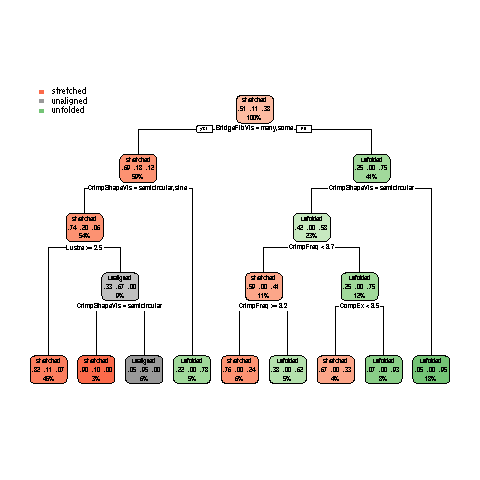
\includegraphics[width=1.1\textwidth]{figrtreeall.png}
  \caption{Binary tree produced by recursive partitioning of 340 sheep data points using all 13 on-sheep scores and measures}
  \label{fig:rtreeall}
\end{figure}

%\end{document}


If we use this tree to predict the 340 sheep in the larning dataset we get
\begin{verbatim}
> prpart.ct3fm <- predict(rpart.ct3fm,may23sf2.df)
> table(predicted=rpred(prpart.ct3fm),actual=may23sf2.df$CrimpTypeFM)
           actual
predicted   stretched unaligned unfolded
  stretched       158        18       20
  unaligned         1        19        0
  unfolded         15         0      109
> 158+19+109
[1] 286
> 286/(286+30+20)
[1] 0.8511905
> 
\end{verbatim}
So 85 percent success. Better than the 78 percent achieved in Watts and Jackson (2017)~\cite{watt:17} with all 10 traits.

The {\em rpart()} function makes a rating of the importance of each variable as follows
\begin{verbatim}
> rpart.ct2fm$variable.importance
 BridgeFibVis CrimpShapeVis        CompEx      StapMaxD      StapArea 
    55.469695     48.394453     32.039403     25.763813     20.591545 
    PeelScore        Lustre     CrimpFreq      Softness       Ringlet 
    18.162290     15.720964     10.086545      7.290892      2.803518 
    Whiteness      StapMinD 
     1.304067      1.148310 
\end{verbatim}
This rating is basically the same as looking at the correlations between the 13 on-sheep scores and the CrimpTypeFMNum varaible shown in Table~\ref{tab:correl}.
There are some variables ( eg PeelScore) which feature high in this list but are not used in the tree. That is because they are measuring the same thing as some other score which is more accurate.

We shall not attempt to prune this 'all-traits' tree, at the moment. In the next section we shall look at  building up a 'simplest-possible' tree starting from one trait. Here we move on to the 'all-traits' approach using discriminant functions.

Discriminant functions require that all the on-sheep traits be numeric. We therefore worj with CrimpShapeVisNum, BridgeFibVisNum, and Ringlet3Num instead of CrimpShapeVis, BridgeFibVis, and Ringlet3. This means that the discriminant function procedure knows the 'ordering' of the three classes for each score, but it is also given an arbitrary spacing of the classes.

We again use all 340 data items, and ignore factors Flock, Age, and Sex. If we use all 13 on-sheep traits , the output from the {\em lda} function is as follows
\begin{verbatim}
> form.ct3fm.lda <- formula(CrimpTypeFM ~ StapMaxD + StapMinD + StapArea + CompEx + Softness + Lustre + Whiteness + PeelScore + CrimpFreq + CrimpShapeVisNum + BridgeFibVisNum +  Ringlet3Num)

> lda.ct3fm <- lda(form.ct3fm.lda,may23sf2.df)
> lda.ct3fm
Call:
lda(form.ct3fm.lda, data = may23sf2.df)

Prior probabilities of groups:
stretched unaligned  unfolded 
0.5123457 0.1111111 0.3765432 

Group means:
          StapMaxD StapMinD  StapArea   CompEx Softness   Lustre Whiteness
stretched 4.522289 2.231928 10.495181 2.933735 3.578313 3.463855  3.373494
unaligned 6.141667 2.738889 18.022222 2.083333 2.444444 2.361111  3.138889
unfolded  3.753279 1.905738  7.514754 3.803279 3.983607 3.754098  3.540984
          PeelScore CrimpFreq CrimpShapeVisNum BridgeFibVisNum Ringlet3Num
stretched  3.638554  3.667470         2.259036        2.018072    1.289157
unaligned  2.750000  4.497222         2.861111        2.777778    1.000000
unfolded   4.352459  3.881148         1.434426        1.180328    1.901639

Coefficients of linear discriminants:
                         LD1         LD2
StapMaxD         -0.20361150  0.52345046
StapMinD          0.33632214  1.64988413
StapArea         -0.02296433 -0.32232225
CompEx            0.30234881 -0.47564542
Softness          0.04119093  0.44784441
Lustre           -0.05441744  0.60614058
Whiteness        -0.19215896 -0.14940269
PeelScore         0.12658837 -0.27785658
CrimpFreq        -0.05893308 -0.32970047
CrimpShapeVisNum -1.04286386  0.16646876
BridgeFibVisNum  -1.00422852  0.08409846
Ringlet3Num       0.23887571 -0.16420746

Proportion of trace:
   LD1    LD2 
0.9155 0.0845 
> 
\end{verbatim}
We see that it makes 2 discriminant functions ( LD1 and LD2 ) and that LD1 consista of 91.5 percent of the between class variance, and LD2 only 8.5 percent. LD1 is dominates by the crimp appearance scores ( CrimpShapeVisNum, BridgeFibVisNum and CompEx), while LD2 is staple size and Lustre.

If we use these 2 functions to predict CrimpTypeFM we achieve the following confusion table
\begin{verbatim}
> plda.ct3fm <- predict(lda.ct3fm,may23sf2.df)
There were 16 warnings (use warnings() to see them)
> table(predicted=plda.ct3fm$class,actual=may23sf2.df$CrimpTypeFM)
           actual
predicted   stretched unaligned unfolded
  stretched       133        14       10
  unaligned         7        22        0
  unfolded         26         0      112
> 133+22+112
[1] 267
> 14+10+7+26
[1] 57
> 267/(267+57)
[1] 0.8240741
> 
\end{verbatim}
So 82 percent success, compared with 79 percent achieved in Watts and Jackson (2017)~\cite{watt:17} with all 10 traits. Not quite as good as the recursive tree partitioning, which is surprising.

The degree to which the two functions (LD1 and LD2) separate the three CrimpTypeFM classes is shown in Figure~\ref{fig:ldaall}
%\documentclass{article}
%\usepackage{graphicx,subfigure}
%\begin{document}

\begin{figure}[!h]
  \centering
  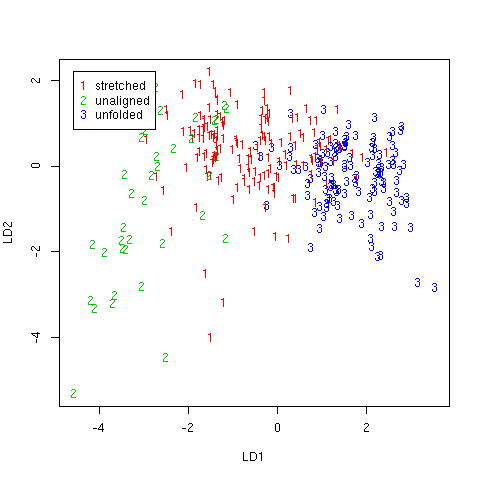
\includegraphics[width=1.1\textwidth]{figldaall.png}
  \caption{Plot of discriminant functions LD1 and LD2 which are the two dimnsions used to discriminate CrimpTypeFM classes. Each point is the LD1 and LD2 function values for one sheep from the learning data set of 340 sheep. The three CrimpType FM classes are shown as colours and numerals}
  \label{fig:ldaall}
\end{figure}

%\end{document}


We can see that there is still not complete separation of the three classes.

We conclude, here, that the 3 new traits (CrimpShapeVis, BridgeFibVis, Ringlet3) plus the revised CrimpTypeFM, have added a little to the success rate of classification, and have adaquately replaced the Ringlet score.

\subsection{Classification using the simplest workable subset of on-sheep traits}
What we want to do here is start with the simplest possible classifier, that is with one trait, and work up towards the smallest set of ttraits which achieve a 'reasonable' success rate. We will define 'reasonable' as around 80 percent success. We will do this for both the recursive tree and the discriminant function approach.

We do not report details of every step. What we report is the success rate for each 'set of traits' bot both techniques. This is given in Table~\ref{tab:success}, starting with one trait and working upwards. 
%\documentclass{article}
%\usepackage{lscape}
%\usepackage{tablefootnote}
%\begin{document}

\begin{table}[htp]
\centering
\caption{Summary of percent success in classifying sheep on CrimpTypeFM with the recursive tree and linear discriminant function techniques. This is a step-up analysis starting with the most important on-sheep trait (CrimpShapeVis) and adding traits one at a time until the the simplest combination of traits that would achieve aroud 80 percent success was found}
\label{tab:success}
\vspace{0.1in}
\begin{tabular}{|p{2.2in}|p{1.2in}|p{1.2in}|}  \hline
  Trait Set & Recursive Tree & Linear Discriminant \\
         & Percent Success & Percent Success  \\ \hline
  CrimpShapeVis               & 72 & 70 \\
  CrimpShapeVis + Ringlet     & 72 & 70 \\
  CrimpShapeVis + CompEx      & 74 & 75 \\
  CompEx                      & 68 & 68 \\
  CrimpShapeVis + StapArea    & 77 & 73 \\
  CrimpShapeVis + StapArea    & & \\
  + CompEx                    & 78 & 78 \\
  StapArea                    & 62 &    \\
  StapMinD                    & 57 &    \\
  StapMaxD                    & 64 &    \\
  CrimpShapeVis + StapMaxD    & 78 & 75 \\
  CrimpShapeVis + StapMaxD    & & \\
  + CompEx                    & 79 & 78 \\
  CrimpShapeVis + Lustre      & 75 & 75 \\
  CrimpShapeVis + Softness    & 74 & 74 \\
  CrimpShapeVis + StapMinD    & 73 & 72 \\
  CrimpShapeVis + BridgeFibVis & 78 & 78 \\
  BridgeFibVis                 & 71 & 69 \\
  CrimpShapeVis + BridgeFibVis & & \\
  +StapMaxD                    & 80 & 78 \\
  CrimpShapeVis + BridgeFibVis & & \\
  + CompEx                     & 81 & 78 \\
  CrimpShapeVis + BridgeFibVis & & \\
  + CompEx +StapMaxD           & 82 & 79 \\
  CrimpShapeVis + BridgeFibVis & & \\
  + CompEx + StapMaxD           & & \\
  + Lustre                     & 83 & 79 \\
  CrimpShapeVis + BridgeFibVis & & \\
  + Lustre                     & & 79 \\
  CrimpShapeVis + BridgeFibVis & & \\
  + Lustre + PeelScore         & & 79 \\
  CrimpShapeVis + BridgeFibVis & & \\
  + Lustre + CrimpFreq         & & 80 \\
  CrimpShapeVis + BridgeFibVis & & \\
  + StapMaxD + CrimpFreq       & & 79 \\
  CrimpShapeVis + BridgeFibVis & & \\
  + CompEx + CrimpFreq         & & 78 \\
\hline 
\end{tabular} 
\end{table}


%\end{document}

What we see is that we can get over 80 percent success with a recursive tree with 3 or 4 traits, two of which should be CrimpShapeVis and BridgeFibVis. THe third trait can be StapMaxD or CompEx.

With linear discriminant functions  we are slightly less successful. The same two traits ( CrimpShapeVis and BridgeFibVis) are essential, and to these we need to add two of ( Lustre, CrimpFreq, or CompEx), and we only get to 79 percent.  hy discriminant functions are slightly less effective is a mystery.

The way that adding one trait at a time grinds the success rate up from 70 percent for one trait to 80 percent for 3 to 4 traits  suggests that what we are dealing with here are random measurement or appraisal errors. As we add more traits the errors tend to cancel and we get more presision in classification. We are probably not adding much new information in adding traits, just cancelling out errors in the same way as we would if we repeat measured/appraised one trait.

\subsection{Predicting numeric CrimpType using multiple regression}

\section{Discussion}
There is not a large difference between the recursive tree approach and the discriminant function approach to classification. The tree approach is limited to considering one trait only at each split, and it draws a cutoff line parallel to the axis for that trait. The discriminant function approach considers all traits at once and only does one split. It is capable of drawing cutoff lines at angles to the axes, and therefore is intrinsically 'better'. It is limited to numeric scores. In practice there is  little difference between the two techniques.

We were able to put some sort of an interpretation on what the various classifiers are doing. From our knowledge of the factors which are important in forming crimp as outlined in Jackson and Watts(2016)~\cite{jack:16}, we were able to intuitively group the visual traits into factors which we called 'alignment', 'space', and 'crimp appearance'. We were able to show that the discriminant functions did something similar. So while the discriminant function analysis is not causal, it does tend to separate the causal factors (space and alignment), but it can not do it completely because there are only 2 discriminant functions, and there are 3 factors involved. The 'crimp appearance' factor tends to  dominate the tree splits, and tends to appear in all discriminant functions, somewhat masking the role of the causal 'align' and 'space' causal factors.

There is a technique called quadratic discriminant functions. We tried it on these data. It  is capable of drawing curved cutoff lines. It was slightly lesss effective than the linear discriminant functions. Results are not reported.

The biggest issue with the present data is that there simply is not a complete separation of the three CrimpTypes, no matter how much statistical manipulation we engage in. We either have to accept that the grading of sheep into three CrimpTypes is an attempt to put 3 classes on a continuum, or we have to search for some further visual observations which might help to better separate the classes. 

It is probably true that the unaligned grade shades into the stretched grade. We may have to live with that. It is the confusion between stretched and unfolded grades that surprises, given that we know that the mechanisms for forming stretched and unfolded crimp are entirely different, and that a given sheep can only be one or the other.

There are mistakes between stretched and unfolded in both directions. Some are what we call 'borderline' cases - the probabilities are close to a 50/50 bet between stretched and unfolded. Others are 'gross mistakes' - the classification procedure is quite sure( ie with a high probability) of its grade, but it is wrong.

We were able to check up on  the CrimpType grades, made by looking for 'twist' on fibre mounts, by looking at the skin data, particularly the IGNorth and IGSouth distances. The grades look to be OK. It is the visual data that are somehow not seeing everything.
 

\begin{thebibliography}{99}

\bibitem{brei:84}
Breiman L., Friedman J.H., Olshen R.A., and Stone C.J. (1984)
Classification and Regression Trees. Wadsworth, California, 1984


\bibitem{jack:16}
Jackson, N. and Watts, J.E. (2016) Staple crimp formation in the fleece of Merino sheep. Unpublished manuscript, 18 May 2016.

\bibitem{onio:62}
Onions, W.J. (1962) Wool: an introduction to its properties, varieties, uses
     and production. Ernest Benn limited, London, 1962

\bibitem{rprog:13}
R Core Team (2013). R: A language and environment for statistical
  computing. R Foundation for Statistical Computing, Vienna, Austria.
  ISBN 3-900051-07-0, URL http://www.R-project.org/.

\bibitem{vena:99}
Venables, W.N. and Ripley, B.D. (1999)
Modern Applied Statistics with S-Plus, 3rd Ed. Springer, New York

\bibitem{watt:17}
Watts, J.M. and Jackson, N. (2017) Classifying sheep into crimp types using on-sheep visual wool scores and measures. Part I. Original crimp type assessment and Zigzag visual crimp scores. Unpublished manuscript, 7 Feb, 2017.

\end{thebibliography}
\end{document}
